%%「論文」,「レター」,「レター(C分冊)」,「技術研究報告」などのテンプレート
%% v3.3 [2020/06/02]


%% 4. 「技術研究報告」
\documentclass[technicalreport,dvipdfmx]{ieicej}
%\usepackage[dvips]{graphicx}
%\usepackage[dvipdfmx]{graphicx,xcolor}
\usepackage[fleqn]{amsmath}
\usepackage{newtxtext}% 英数字フォントの設定を変更しないでください
\usepackage[varg]{newtxmath}% % 英数字フォントの設定を変更しないでください
\usepackage{latexsym}
%\usepackage{amssymb}
\usepackage[dvipdfmx]{graphicx}

\jtitle{}
\jsubtitle{}
\etitle{}
\esubtitle{}
\authorlist{%
 \authorentry[]{}{}{}
% \authorentry[メールアドレス]{和文著者名}{英文著者名}{所属ラベル}
}
\affiliate[]{}{}
%\affiliate[所属ラベル]{和文勤務先\\ 連絡先住所}{英文勤務先\\ 英文連絡先住所}
\jalcdoi{???????????}% ← このままにしておいてください

\begin{document}
\begin{jabstract}
%和文あらまし
\end{jabstract}
\begin{jkeyword}
%和文キーワード
\end{jkeyword}
\begin{eabstract}
%英文アブストラクト
\end{eabstract}
\begin{ekeyword}
%英文キーワード
\end{ekeyword}
\maketitle

\section{はじめに}
日本は災害大国であり,毎年大規模な自然災害が発生している. 近年では,いわゆる異常気象による豪雨により甚大な被害が発生しており,命を落とす人も後を絶たない. 2018年7月の西日本で発生した豪雨災害では,死者200人を超える被害が出た[参考文献].犠牲者が出た地域の多くは,洪水浸水想定区域や土砂災害警戒区域内であり,避難行動を促す情報が事前に発令されていた. つまり,特に豪雨災害においては,住民が逃げ遅れによって死亡している事例が多い. 逃げ遅れの主な要因は,「自分は大丈夫だ」と思い込む正常性バイアス等の心理効果による避難意識の欠如,災害時における適切な行動が分からないなどの知識不足,避難場所の確認不足などが挙げられる[参考文献].
さらに2020年に起こった新型コロナウイルス感染症の流行によって,感染対策を考慮した新たな避難所運営が必要になっている[参考文献].その一環として,三密回避のための避難所の受け入れ人数制限・管理があり,避難してきた住民が避難所に入れなくなる事態が想定される.実際に2020年9月九州に台風10号が直撃し避難所が開設された際に,避難してきた住民が2か所続けて受入拒否された事例が発生している[参考文献]. 
このような問題に対して,独自に対策を行なっている自治体もある. 宮崎県日南市では,飲食店などの混雑状況を配信するアプリケーションVACANを用いて,避難所の混雑状況の配信を行い,一定の効果を上げている[参考文献].しかしながら,避難所の混雑状況は,自治体職員の手作業によって計測・更新されている.したがって,コロナ時代に必要な新たな施策も,各自治体に任せきりになっており,職員の職務負担の増大につながっているのが現状である.
このような背景の下,我々は「コロナ時代に災害が起きた場合,住民が自治体に頼ることなく,自分たちで適切な避難所へ分散避難できないか?」をリサーチクエスチョンに設定して研究を進めている.
本研究では,住民の自助によって避難所での密の形成を回避し,迅速且つ安全な避難の実現を支援するモバイル・アプリケーションShelter Naviを提案する. Shelter Naviは,クラウドサーバで自治体内の避難所の場所と混雑状態を管理し,地図上に可視化して,災害時に住民が密を避けて分散避難するための情報を提供する.住民が避難所に「チェックイン」すると,Shelter Naviは混雑度合いをリアルタイムに更新する.これによって,各避難所に特別な設備を必要とすることなく,避難所での密を考慮した避難が可能となる.
本稿では,Shelter Naviのユースケースを定義し,ドメインモデルおよびサービスの設計を行う.さらに,Shelter NaviのプロトタイプをSpring Boot [参考文献]およびBootstrapを活用したモバイルWebアプリケーションとして実装する.Shelter Naviによって,住民の避難意識の向上と,With/Afterコロナ時代の避難所運営の効率化につながることが期待できる.

\section{準備}
\subsection{日本における災害避難} 
近年わが国では,異常気象などの影響により「数十年に一度」と言われるような大規模な豪雨災害が頻繁に発生しており,毎年多くの犠牲者が発生している. 2018年7月の西日本豪雨災害では,避難勧告が発令されていたにもかかわらず,人的被害が多く発生したことが報告されている.[1] 犠牲者の中には「逃げ遅れ」によるものが多く存在した.
災害時における住民の避難を促すための情報として,気象庁から発令される大雨・暴風・洪水等の気象警報,各自治体から発令される避難勧告並びに避難指示等がある. 避難指示に関しては,強制力はないため,避難するかどうかは,避難することによる危険などを踏まえた住民の判断に任されている. しかし,このような自身の身に危険が迫っている場合は,大量の情報の処理を時間的制約がある中で正確に行うことを迫られることなどによる強いストレスにより,冷静さを保つ目的で,平常時と同じリスク評価,つまり事態を楽観視してしまう傾向である「平常性バイアス」が働く. これにより,自身に都合の良いように解釈をしてしまい,「自分は大丈夫だ」といったような思考が生まれ,結果として意思決定や避難行動の遅れにつながっていると考えられている. [2] 加えて,避難する避難所の確認ができていない,避難経路がわからないなどの住民の事前準備や意識の低さも避難率の低下につながっている.

\subsection{コロナ時代の避難所運営}
2020年,新型コロナウイルス感染症の世界的流行により,社会のあらゆる場面で様式の変化が求められた. 防災の面では,避難所での感染対策が急務で進められ,各自治体から感染対策が盛り込まれた新たな避難所運営マニュアルが発行された. 具体的には,避難スペースの設置レイアウト例(収容人数,間隔など)や避難所受け入れ前の検温・問診などの実施などが新たに示された. また,密集を避けるため,避難所当たりの収容人数を大きく制限せざるをえなくなった.
このような感染対策により,状況がわからずに避難してきた住民が避難所に入れてもらえないケースが懸念されている.2020年9月九州に台風10号が直撃し避難所が開設された際に,避難してきた住民が2か所続けて受入拒否された事例が発生している[参考文献]. 
このような問題に対し,独自に対策を行なっている自治体もある.宮前県日南市では,飲食店の混雑状況などを配信するアプリケーション「VACAN」を用いて,避難所の混雑状況の配信を行っている.しかしながら,避難所の混雑状況は,自治体職員の手作業によって計測・更新されている.
このように,コロナ時代における避難所運営の新たな施策も試行錯誤的に行われてきているが,基本的には自治体に任せきりになっており,職員の職務負担の増大につながっているのが現状である.さらには,このような自治体の対策に住民が依存してしまい,住民の自助が抑制されてしまうことも懸念される. 

\subsection{リサーチクエスチョン}
以上を踏まえて,我々は以下のリサーチクエスチョンを設定し,それに答える手法を研究している.

\begin{itemize}
     \item{\textbf{RQ}「コロナ時代に災害が起きた場合,住民が自治体に頼ることなく,自分たちで適切な避難所へ分散避難できないか?」}
\end{itemize}

\section{提案手法}
\subsection{システム概要}

\subsection{ユースケース}

\subsection{システムアーキテクチャ}

\subsection{ドメインモデリング}
ShelterNaviにおけるドメインモデル図\ref{fig:domain}にを示す.
ShelterNaviには,図\ref{fig:domain}で表されている5つのドメインが存在し,それぞれShelter(避難所),User(住民・ユーザ),Check-In(避難所へのチェックインまたはチェックアウト),ShelterState(避難所の状態),UserState(ユーザの状態)となっている.Check-Inドメインを通じてユーザとそのユーザが利用した避難所を関連付けさせるために,Check-Inドメインは必ず1つのUserドメインと1つのShelterドメインと結びつく.また,ShelterStateドメインは各避難所の状態を表しており,UserStateドメインはユーザの避難状態を示している.
以下では,ShelterNaviの各ドメインを構成する要素について説明する.Shelterドメインにおいては,システムがどの避難所か特定するためのIDが必要であり,避難するユーザに向けて避難所の名称,位置情報を示す必要がある.そして,避難所の開放情報も取り扱う.以上のことからShelterドメインでは以下のスキーマを規定する.

\begin{itemize}
    \item{\textbf{sid:}}避難所ID
    \item{\textbf{name:}}避難所の名称
    \item{\textbf{address:}}避難所の住所
    \item{\textbf{lat:}}避難所の緯度
    \item{\textbf{lng:}}避難所の経度
    \item{\textbf{capacity:}}避難所の収容可能人数
    \item{\textbf{isActive:}}避難所が利用可能か
\end{itemize}

続いてUserドメインにおいては,ユーザ情報を一意に取り扱うためのユーザIDが必要である.また,本サービスに登録するためのemailアドレスとパスワード,(名前,住所:必要性をどう示すか),そして混雑度を計算するための世帯人数を取り扱う.% 本アプリにおける名前,住所,電話番号の必要性
以上のことからUserドメインでは以下のスキーマを規定する.

\begin{itemize}
    \item{\textbf{uid:}}ユーザID
    \item{\textbf{email:}}メールアドレス
    \item{\textbf{password:}}パスワード
    \item{\textbf{name:}}ユーザの名前
    \item{\textbf{address:}}ユーザの住所
    \item{\textbf{of families:}}世帯人数
\end{itemize}

Check-Inドメインにおいては,どのユーザがどの避難所を利用しているかを管理するためにユーザIDと避難所IDが必要である.また,複数の避難所への多重チェックインがないかを確認するために,チェックイン時刻と,チェックアウト時刻も取り扱う.以上のことからCheck-Inドメインでは以下のスキーマを規定する.

\begin{itemize}
    \item{\textbf{cid:}}チェックインID
    \item{\textbf{uid:}}ユーザID
    \item{\textbf{sid:}}避難所ID
    \item{\textbf{checkin-datetime:}}チェックイン時刻
    \item{\textbf{checkout-datetime:}}チェックアウト時刻
\end{itemize}

ShelterStateドメインにおいては,コロナ禍における避難所での密を考慮すべく,避難所の混雑度も取り扱う.この混雑度は,避難所の収容可能人数に対しての現在の収容人数の割合から求められるので収容人数も管理する.そしてチェックイン,チェックアウトによる収容人数の変化を見るために,避難所の状態の最終更新日時も取り扱う.以上のことからShelterStateドメインでは以下のスキーマを規定する.

% 現在の収容人数のスキーマ名なににするべきか...
\begin{itemize}
     \item{\textbf{id:}}避難所の状態ID
     \item{\textbf{sid:}}避難所ID
     \item{\textbf{num of accomodated:}}収容人数
     \item{\textbf{congestion:}}混雑度
     \item{\textbf{changedAt:}}更新日時
 \end{itemize}

UserStateドメインでは,ユーザの避難状態の履歴を管理する.特定のユーザの履歴を見るためにユーザIDが必要である.そして,準備中,避難済み等の避難状態を表すスキーマを取り扱い,避難状態が変化した際の日時を記録する.なお,このUserStateドメインでは過去のデータを参照できるようにしておくために,1つのデータを更新していくのではなく,新規データを追加していく形をとる.

 \begin{itemize}
     \item{\textbf{id:}}ユーザの状態ID
     \item{\textbf{uid:}}ユーザID
     \item{\textbf{state:}}避難状態
     \item{\textbf{changedAt:}}更新日時
 \end{itemize}

\begin{figure}[htbp]
     \begin{center}
          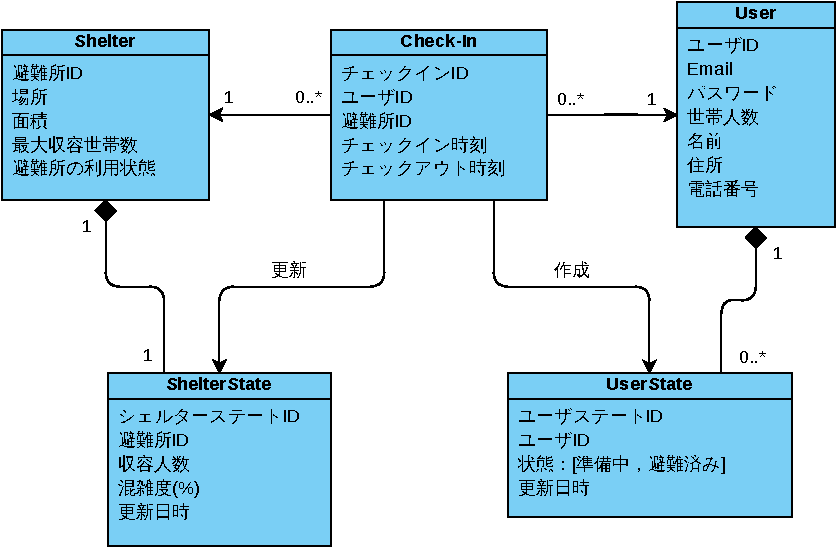
\includegraphics[scale=0.5,pagebox=cropbox,clip]{domain_model.pdf}
          \caption{ドメインモデル図}
          \label{fig:domain}
     \end{center}
\end{figure}
% CitizenStateドメインではユーザの状態しか取り扱わない?
% Citizenドメインのフィールドとするのはダメなのかチェックする

\subsection{主要なサービス}
\label{sec:service}
ShelterNaviでは他のアプリケーションとの連携や拡張性を考慮し,HTTPを介して外部から利用できるAPIを配備した.以下にAPIの詳細を示す.

\subsubsection{シェルターサービス}
\begin{itemize}
    \item{\textbf{createShelter( shelterForm ):}
         避難所ID,避難所名,位置情報を基に避難所データを作成し,取得する.}
    \item{\textbf{getShelter( sid ):}
         避難所IDを指定することで該当する避難所データを取得する.}
    \item{\textbf{deleteShelter( sid ):}
         避難所IDを指定することで該当する避難所データを削除する.}
    \item{\textbf{clearAllShelters():}
         全ての避難所データを削除する.}
    \item{\textbf{getAllShelters():}
         全ての避難所データを取得する.}
    \item{\textbf{searchSheltersByDistance( lng, lat, distance ):}
         経度,緯度,そして距離を指定することで,指定位置座標(lng, lat)から半径distance$\rm[km]$以内にある避難所データ全てを取得する.当APIでは,地球上における大圏(大円)距離を計算する手法を使用しており,地球の半径を6371[km],ユーザの経度座標をlng,緯度座標をlat,各避難所データの経度座標をs\_lng,緯度座標をs\_latとし,ユーザから半径distance[km]以内に存在する避難所を検索するものとして以下の計算式を用いる.

         \begin{eqnarray*}
             6371 \arccos ( \cos( radians( lat ) ) \times \cos( radians( s\_lat ) ) \\
             \times \cos( radians( s\_lng ) - radians( lng ) ) + \sin( radians( lat ) ) \\
             \times \sin( radians( s\_lat ) ) ) \leqq distance
         \end{eqnarray*}}
    \item{\textbf{searchSheltersByKeyword( keyword ):}
         文字列を指定することで,全避難所データの避難所名,または避難所の住所に部分一致するものがないか検索し,該当するデータを全て取得する.}
\end{itemize}

\subsubsection{ユーザサービス}
\begin{itemize}
    \item{\textbf{createUser( userForm ):}
         メールアドレス,パスワード,世帯人数等のユーザ情報を元に新規アカウントを作成し,取得する.}
    \item{\textbf{getUser( uid ):}
         ユーザIDを指定することで該当するユーザアカウントを取得する.}
    \item{\textbf{deleteUser( uid ):}
         ユーザIDを指定することで該当するユーザアカウントを削除する.}
\end{itemize}

\subsubsection{チェックインサービス}
\begin{itemize}
    \item{\textbf{checkIn( uid, sid ):}
         ユーザIDと避難所IDを指定することで,チェックインデータを作成し,更新日時を記録する.}
    \item{\textbf{checkOut( uid, sid ):}
         ユーザIDと避難所IDから一意に定まるチェックインデータを取得し,チェックアウト時刻を更新する.}
\end{itemize}

\subsubsection{シェルターステートサービス}
\begin{itemize}
     \item{\textbf{checkIn( uid, sid ):}
          ユーザIDと避難所IDを指定することで,避難所の収容人数をユーザの世帯人数分増加させ,避難所の混雑度を計算し,更新する.また,更新日時を記録する.}
     \item{\textbf{checkOut( uid, sid ):}
          ユーザIDと避難所IDを指定することで,避難所の収容人数をユーザの世帯人数分減少させ,避難所の混雑度を計算し,更新する.また,更新日時を記録する.}
\end{itemize}

\subsubsection{ユーザステートサービス}
\begin{itemize}
     \item{\textbf{checkIn( uid ):}
          ユーザIDを指定することで,特定のユーザの避難状態を「避難済み」にしたUserStateのデータを新規で作成する.また,更新日時も併せて記録する.}
     \item{\textbf{checkOut( uid ):}
          ユーザIDを指定することで,特定のユーザの避難状態を「準備中」にしたUserStateのデータを新規で作成する.また,更新日時も併せて記録する.}
\end{itemize}

\section{実装}
\subsection{ShelterNaviプロトタイプの実装}
今回は以下の開発環境で「ユーザサービス」,「シェルターサービス」,また「チェックインサービス」の一部の開発を行った.
\begin{itemize}
    \item サーバ開発言語:Java
    \item クライアント開発言語:HTML5,JavaScript
    \item CSSライブラリ:BootStrap
    \item データベース:MySQL 8.0.20
    \item Webサーバ:Apache Tomcat
    \item Webサービスフレームワーク:SpringBoot(Java)
\end{itemize}
以下ではShelterNaviの「サインアップ」,「ログイン」,「避難所検索」,「チェックイン」の各画面構成に併せて実装の詳細を述べる.

\subsection{サインアップ}
\label{sec:signup}
サインアップ画面を図\ref{fig:signup}に示す.サインアップ画面は,ログイン時に必要なメールアドレスとパスワードからなる「ログイン情報」とログイン後,システム内で扱われる名前,住所,世帯人数,電話番号(任意)からなる「個人情報」の2つの要素で構成されている.これらの情報を入力したうえで図\ref{fig:signup}下部の登録ボタンをクリックすれば,ユーザ新規登録の完了となる.

\subsection{ログイン}
ログイン画面を図\ref{fig:login}に示す.ログイン画面では\ref{sec:signup}で述べた「ログイン情報」であるメールアドレスとパスワードを画面中央にある項目に入力し,ログインボタンをクリックする.ユーザとして登録済みの正しいメールアドレスとパスワードが入力できていれば,ログイン後に避難所検索画面に移行する.ログインが成功した際は,ユーザごとに権限が与えられる仕組みになっており,通常付与される権限では\ref{sec:service}で紹介したAPIの一部しか扱えないため,自身の登録した情報が他ユーザから閲覧,更新,削除されることはない.
%今回の実装においては,セキュリティ性を担保するためにJavaのフレームワークであるSpring Securityを用いる.このフレームワークの機能を利用すれば,指定したURL内で,IDとパスワードをPostする特定のAPIを利用することで認証が可能になる.また,ユーザオブジェクトに権限を付与し,その権限に応じた認可を与えることも可能になる.本アプリケーションでは,通常の工程でユーザを作成した場合,CITIZEN(住民・一般ユーザ)の役割が付与される.実際には,ログイン機能における認証時にこの役割を見ることで,セッションに対して役割に対応した権限を付与する.これによりログイン後のユーザに対する各ページへの認可が可能になる.

\subsection{避難所検索}
%実際は管理者が直接データを入れることになりそうなので機能ではない?

\subsection{チェックイン}
%本アプリケーションでは,避難所を可視化する上でGoogle Mapを利用している.避難所を取得するAPIで避難所データを取得し,それらのデータをGoogleMapsAPIで利用することで,地図上への避難所の可視化を行っている.また,ShelterNaviではユーザの現在位置に応じて地図上に表示する避難所を変更しており,これは「3.5 主要なサービス」で言及したsearchSheltersByDistance(lng, lat, distance)をを利用している.

\begin{figure}[htbp]
     \begin{center}
          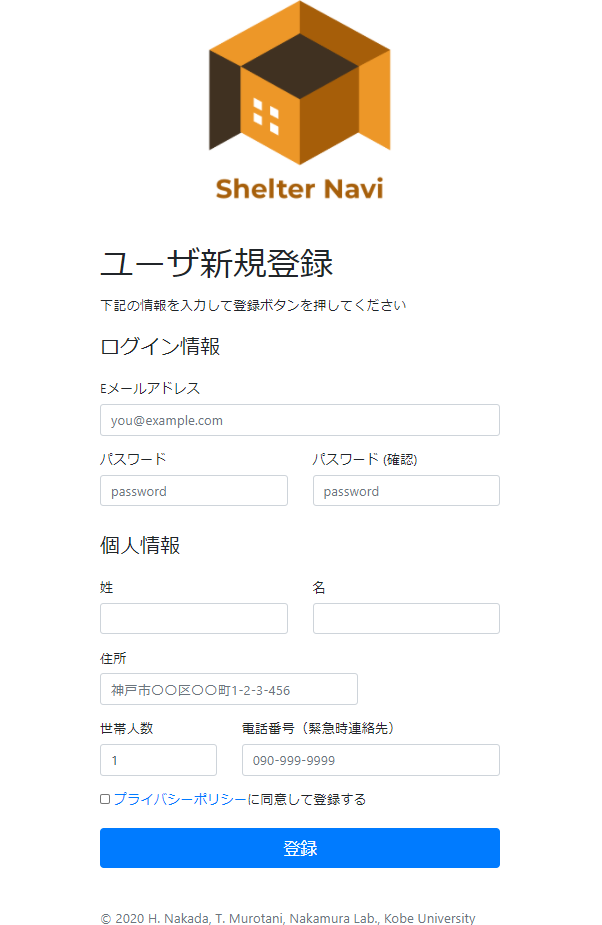
\includegraphics[scale=0.5,pagebox=cropbox,clip]{signup.png}
          \caption{新規登録画面}
          \label{fig:signup}
     \end{center}
\end{figure}

\begin{figure}[htbp]
     \begin{center}
          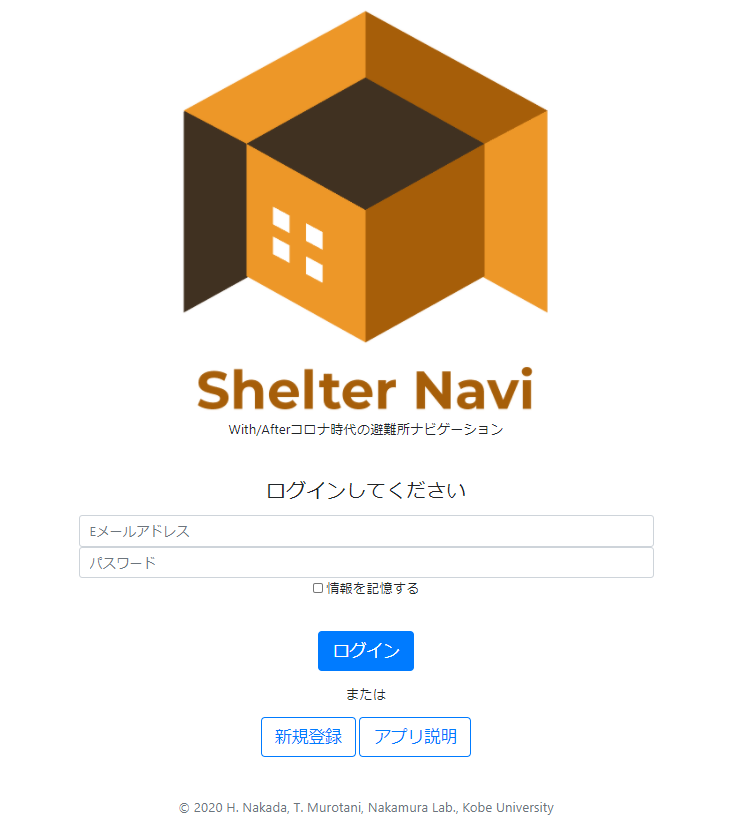
\includegraphics[scale=0.5,pagebox=cropbox,clip]{login.png}
          \caption{ログイン画面}
          \label{fig:login}
     \end{center}
\end{figure}

\begin{figure}[htbp]
     \begin{center}
          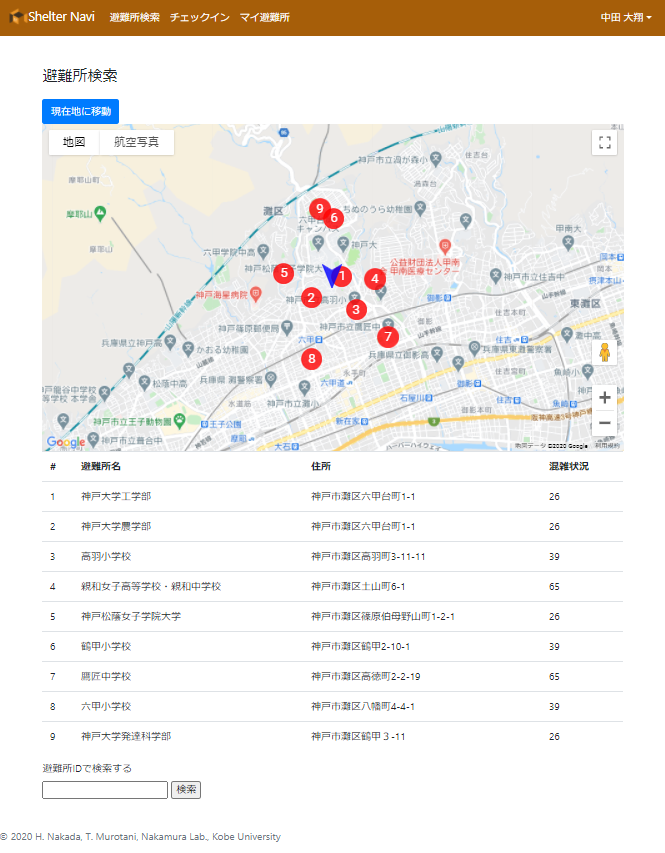
\includegraphics[scale=0.6,pagebox=cropbox,clip]{search_shelter.png}
          \caption{避難所検索画面}
          \label{fig:search_shelter}
     \end{center}
\end{figure}

\section{考察・評価}

\section{おわりに}


%\bibliographystyle{sieicej}
%\bibliography{myrefs}
\begin{thebibliography}{99}% 文献数が10未満の時 {9}
\bibitem{}
\end{thebibliography}

\end{document}


%% 1. 「論文」
\documentclass[paper]{ieicej}
%\documentclass[invited]{ieicej}% 招待論文
%\documentclass[survey]{ieicej}% サーベイ論文
%\documentclass[comment]{ieicej}% 解説論文
%\usepackage[dvips]{graphicx}
%\usepackage[dvipdfmx]{graphicx,xcolor}
\usepackage[fleqn]{amsmath}
\usepackage{newtxtext}% 英数字フォントの設定を変更しないでください
\usepackage[varg]{newtxmath}% % 英数字フォントの設定を変更しないでください
\usepackage{latexsym}
%\usepackage{amssymb}

\setcounter{page}{1}

\field{}
\jtitle{}
\etitle{}
\authorlist{%
 \authorentry{}{}{}\MembershipNumber{}
 %\authorentry{和文著者名}{英文著者名}{所属ラベル}\MembershipNumber{}
 %\authorentry[メールアドレス]{和文著者名}{英文著者名}{所属ラベル}\MembershipNumber{}
 %\authorentry{和文著者名}{英文著者名}{所属ラベル}[現在の所属ラベル]\MembershipNumber{}
}
\affiliate[]{}{}
%\affiliate[所属ラベル]{和文所属}{英文所属}
%\paffiliate[]{}
%\paffiliate[現在の所属ラベル]{和文所属}
\jalcdoi{???????????}% ← このままにしておいてください

\begin{document}
\begin{abstract}
%和文あらまし 500字以内
\end{abstract}
\begin{keyword}
%和文キーワード 4〜5語
\end{keyword}
\begin{eabstract}
%英文アブストラクト 100 words
\end{eabstract}
\begin{ekeyword}
%英文キーワード
\end{ekeyword}
\maketitle



\ack %% 謝辞

%\bibliographystyle{sieicej}
%\bibliography{myrefs}
\begin{thebibliography}{99}% 文献数が10未満の時 {9}
\bibitem{}
\end{thebibliography}

\appendix

\begin{biography}
\profile{}{}{}
%\profile{会員種別}{名前}{紹介文}% 顔写真あり
%\profile*{会員種別}{名前}{紹介文}% 顔写真なし
\end{biography}

\end{document}



%% 2. 「レター」
\documentclass[letter]{ieicej}
%\usepackage[dvips]{graphicx}
%\usepackage[dvipdfmx]{graphicx,xcolor}
\usepackage[fleqn]{amsmath}
\usepackage{newtxtext}% 英数字フォントの設定を変更しないでください
\usepackage[varg]{newtxmath}% % 英数字フォントの設定を変更しないでください
\usepackage{latexsym}
%\usepackage{amssymb}

\setcounter{page}{1}

\typeofletter{研究速報}
%\typeofletter{紙上討論}
%\typeofletter{問題提起}
%\typeofletter{ショートノート}
\field{}
\jtitle{}
\etitle{}
\authorlist{%
 \authorentry{}{}{}{}\MembershipNumber{}
 %\authorentry{和文著者名}{英文著者名}{会員種別}{所属ラベル}\MembershipNumber{}
 %\authorentry{和文著者名}{英文著者名}{会員種別}{所属ラベル}[現在の所属ラベル]\MembershipNumber{}
}
\affiliate[]{}{}
%\affiliate[所属ラベル]{和文所属}{英文所属}
%\paffiliate[]{}
%\paffiliate[現在の所属ラベル]{和文所属}
\jalcdoi{???????????}% ← このままにしておいてください

\begin{document}
\maketitle
\begin{abstract}
%和文あらまし 120字以内
\end{abstract}
\begin{keyword}
%和文キーワード 4〜5語
\end{keyword}
\begin{eabstract}
%英文アブストラクト 50 words
\end{eabstract}
\begin{ekeyword}
%英文キーワード
\end{ekeyword}

\section{まえがき}


\ack %% 謝辞

%\bibliographystyle{sieicej}
%\bibliography{myrefs}
\begin{thebibliography}{99}% 文献数が10未満の時 {9}
\bibitem{}
\end{thebibliography}

\appendix
\section{}

\end{document}


%% 3. 「レター(C分冊)」
\documentclass[electronicsletter]{ieicej}
%\usepackage[dvips]{graphicx}
%\usepackage[dvipdfmx]{graphicx,xcolor}
\usepackage[fleqn]{amsmath}
\usepackage{newtxtext}% 英数字フォントの設定を変更しないでください
\usepackage[varg]{newtxmath}% % 英数字フォントの設定を変更しないでください
\usepackage{latexsym}
%\usepackage{amssymb}

\setcounter{page}{1}

\field{}
\jtitle{}
\etitle{}
\authorlist{%
 \authorentry{}{}{}{}\MembershipNumber{}
 %\authorentry{和文著者名}{英文著者名}{会員種別}{所属ラベル}\MembershipNumber{}
 %\authorentry{和文著者名}{英文著者名}{会員種別}{所属ラベル}[現在の所属ラベル]\MembershipNumber{}
}
\affiliate[]{}{}
%\affiliate[所属ラベル]{和文所属}{英文所属}
%\paffiliate[]{}
%\paffiliate[現在の所属ラベル]{和文所属}
\jalcdoi{???????????}% ← このままにしておいてください

\begin{document}
\begin{abstract}
%和文あらまし 120字以内
\end{abstract}
\begin{keyword}
%和文キーワード 4〜5語
\end{keyword}
\begin{eabstract}
%英文アブストラクト 50 words
\end{eabstract}
\begin{ekeyword}
%英文キーワード
\end{ekeyword}
\maketitle

\section{まえがき}


\ack %% 謝辞

%\bibliographystyle{sieicej}
%\bibliography{myrefs}
\begin{thebibliography}{99}% 文献数が 10 未満の時 {9}
\bibitem{}
\end{thebibliography}

\appendix
\section{}

\end{document}
